% Chapter 4: Design and Implementation

\chapter{Diseño e implementación} % Main chapter title

\label{Chapter4} % Reference

%-------------------------------------------------------------------------------

\section{Arquitectura de seguridad}

Para entender la arquitectura de seguridad de la aplicación, es importante distinguir entre las siguientes propiedades de la seguridad de la información: confidencialidad, integridad y autenticación.

\subsection{Confidencialidad}

Para el cifrado de la información se utiliza criptografía de clave simétrica, ya que ofrece una mayor velocidad de cifrado frente a otros modelos. Debido a que puede funcionar tanto sobre \emph{hardware} como sobre \emph{software}, a que es un estándar del cifrado simétrico y a que no tiene debilidades conocidas, AES es el algoritmo de cifrado simétrico que se utiliza en esta aplicación. (Véase~\ref{AES})

De entre todos los tamaños de clave disponibles se ha optado por el de 128 \emph{bits}, ya que ofrece un nivel de seguridad adecuado para la aplicación. Además, un nivel superior habría supuesto una mayor carga computacional.

Igualmente, es necesario cifrar la clave simétrica utilizada. Para ello se utiliza un sistema de cifrado asimétrico para proteger la clave. Debido otra vez a que es un estándar, se utiliza RSA como algoritmo de cifrado asimétrico. (Véase~\ref{RSA})

Ya que el número de operaciones de cifrado asimétrico es menor que el del simétrico, se utiliza el tamaño máximo para una clave RSA: 4096 \emph{bits}.

\subsection{Integridad}

También es importante que el mensaje permanezca íntegro. Para ello se incluye junto con el mensaje una HMAC. (Véase~\ref{HMAC})

De entre algunos algoritmos de codificación se ha decidido utilizar PSS. Este algoritmo, entre otras cosas, combina el uso de una \emph{salt} con un resumen \emph{hash}, lo cual lo hace más robusto frente a determinados ataques enfocados en la obtención del mensaje original a partir de su resumen. (Véase~\ref{PSS})

\subsection{Autenticación}

El destinatario tiene que poder autenticar al autor del mensaje. Para lograrlo se incluye junto al mensaje una HMAC. (Véase~\ref{HMAC})

Se utiliza como algoritmo de firma RSASSA-PSS, ya que combina los algoritmos utilizados para preservar la confidencialidad y la integridad. Este algoritmo genera un mensaje codificado a partir del resumen del mensaje original, utilizando para ello PSS, y luego firma (cifra) este mensaje usando RSA. (Véase~\ref{RSASSA-PSS})

Para proporcionar confidencialidad a la firma, esta va cifrada usando la clave pública del destinatario, de forma que nadie más pueda acceder a su contenido.

%-------------------------------------------------------------------------------

\section{Arquitectura del software}

El objetivo de este \emph{software} es proporcionar una herramienta que permita a los usuarios mantener comunicaciones con otros usuarios preservando las tres propiedades de la seguridad comentadas en el punto anterior. Para ello, se ha llevado a cabo el desarrollo de varios prototipos:

\begin{itemize}
  \item El primer prototipo sienta las bases de la arquitectura de orientación a objetos que utiliza la aplicación. Posee un esquema que recibe un fichero y lo divide en varios fragmentos de un tamaño dado, almacenando estos fragmentos en estructuras de datos. También puede recomponer el fichero original a partir de los fragmentos.

  \item El segundo prototipo realiza las mismas tareas que el anterior, y además añade confidencialidad a los fragmentos mediante un sistema de cifrado simétrico.

  \item El tercer prototipo realiza las mismas tareas que el anterior, y además añade el uso de RSA para cifrar claves simétricas y proporcionar integridad y autenticación a los fragmentos.

  \item El cuarto prototipo realiza las mismas tareas que el anterior, ahora como una aplicación en Android. Se añade una interfaz gráfica y hace uso de algunas herramientas que posee Android para el almacenamiento de claves.
\end{itemize}

\subsection{Shatter I}

El primer prototipo de la aplicación está desarrollado enteramente en Java, usando para ello el entorno de desarrollo Eclipse. Esta primera versión busca poder dividir un fichero en varios fragmentos de un tamaño dado, y luego poder recomponerlo. Para ello se han implementado algunas clases para almacenar los datos de los fragmentos:

\begin{figure}[!htb]
  \centering
  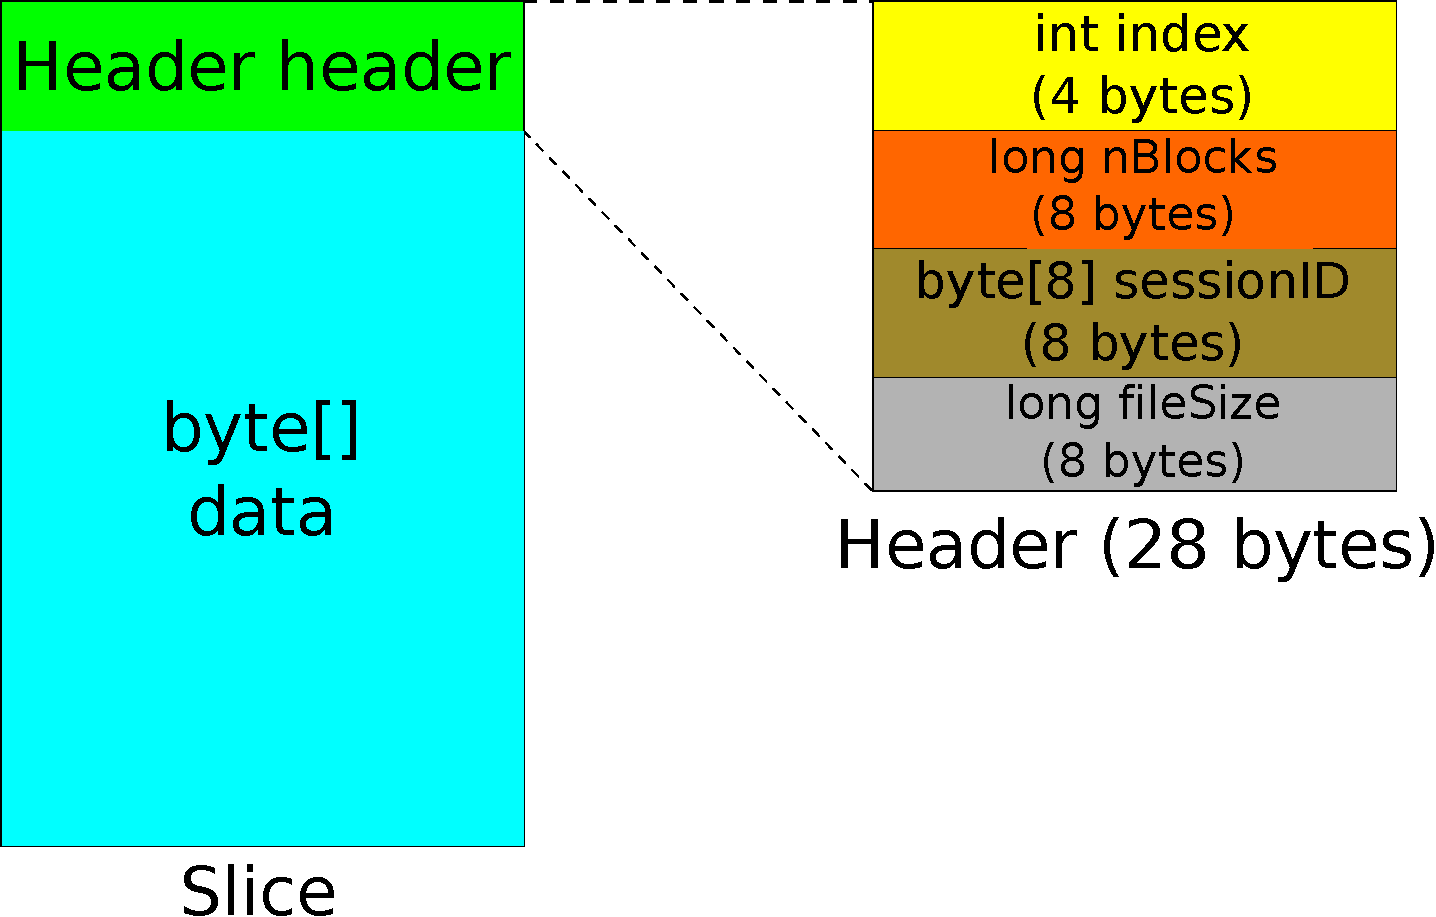
\includegraphics[scale=0.4]{Figures/Slice_Header_1}
  \decoRule
  \caption[\code{Slice} - \code{Header} (Versión 1)]{Esquema general de las clases \code{Slice} y \code{Header} (Versión 1)}
  \label{fig:Slice_Header_1}
\end{figure}

\begin{itemize}
  \item \keyword{\code{Slice}} -- Un objeto de clase \code{Slice} es uno de los fragmentos en los que un fichero original se ha dividido. Está formado por una cabecera (\code{Header}) y un array de \emph{bytes} en el que se almacena el contenido del segmento del fichero. (Figura~\ref{fig:Slice_Header_1}) \footnote{Debido al contexto del TFG, se ha decidido no usar UML para confeccionar los esquemas expuestos en este capítulo.}

  \item \keyword{\code{Header}} -- En esta clase se almacenan los metadatos de un objeto de clase \code{Slice}. Se guardan datos como un contador, el número total de fragmentos para un fichero, un ID para la sesión\footnote{En esta primera iteración de la aplicación, el ID para identificar la sesión es un resumen \emph{hash} del fichero.} y el tamaño original del fichero. (Figura~\ref{fig:Slice_Header_1})
\end{itemize}

También se han desarrollado otras clases con métodos para trocear y recomponer un fichero:

\begin{figure}[!htb]
  \centering
  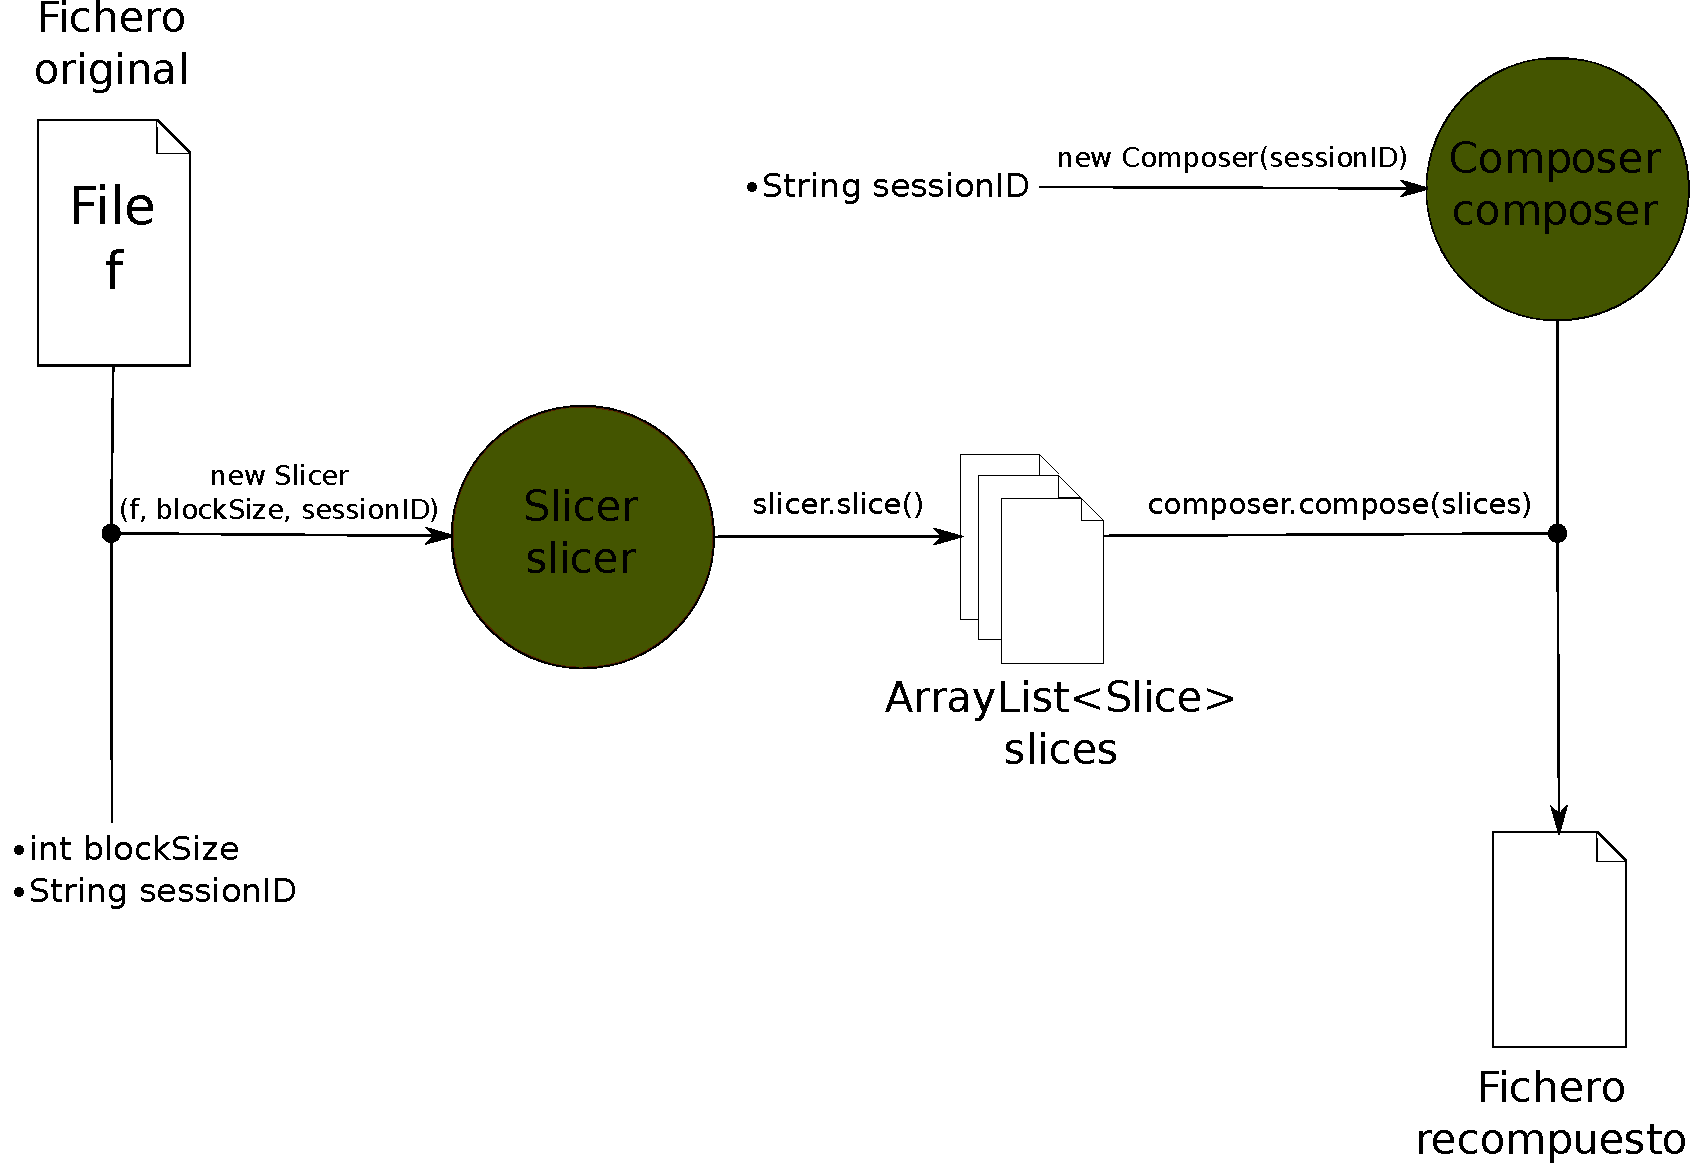
\includegraphics[scale=0.5]{Figures/Assembler}
  \decoRule
  \caption[\code{Slicer} - \code{Composer}]{Esquema general del funcionamiento de las clases \code{Slicer} y \code{Composer}}
  \label{fig:Assembler}
\end{figure}

\begin{itemize}
  \item \keyword{\code{Slicer}} -- Esta clase posee métodos para crear objetos de clase \code{Slice}. Recibe un fichero, un tamaño de bloque y un ID para identificar la sesión. Lee del fichero bloques del tamaño indicado hasta alcanzar el EOF y genera un \code{Slice} para cada uno de ellos, con una cabecera distinta. (Figura~\ref{fig:Assembler})

  \item \keyword{\code{Composer}} -- Esta clase, a través de un método, recibe un array de objetos de clase \code{Slice} y devuelve un fichero compuesto. Lee uno a uno los fragmentos que recibe, prestando especial atención a sus cabeceras y si detecta que alguno falta genera un log de errores. (Figura~\ref{fig:Assembler})
\end{itemize}

\subsection{Shatter II}

En esta segunda versión, el objetivo del prototipo es proporcionar confidencialidad a los objetos de clase \code{Slice}. Para llevarlo a cabo se han implementado las siguientes clases:

\begin{figure}[!htb]
  \centering
  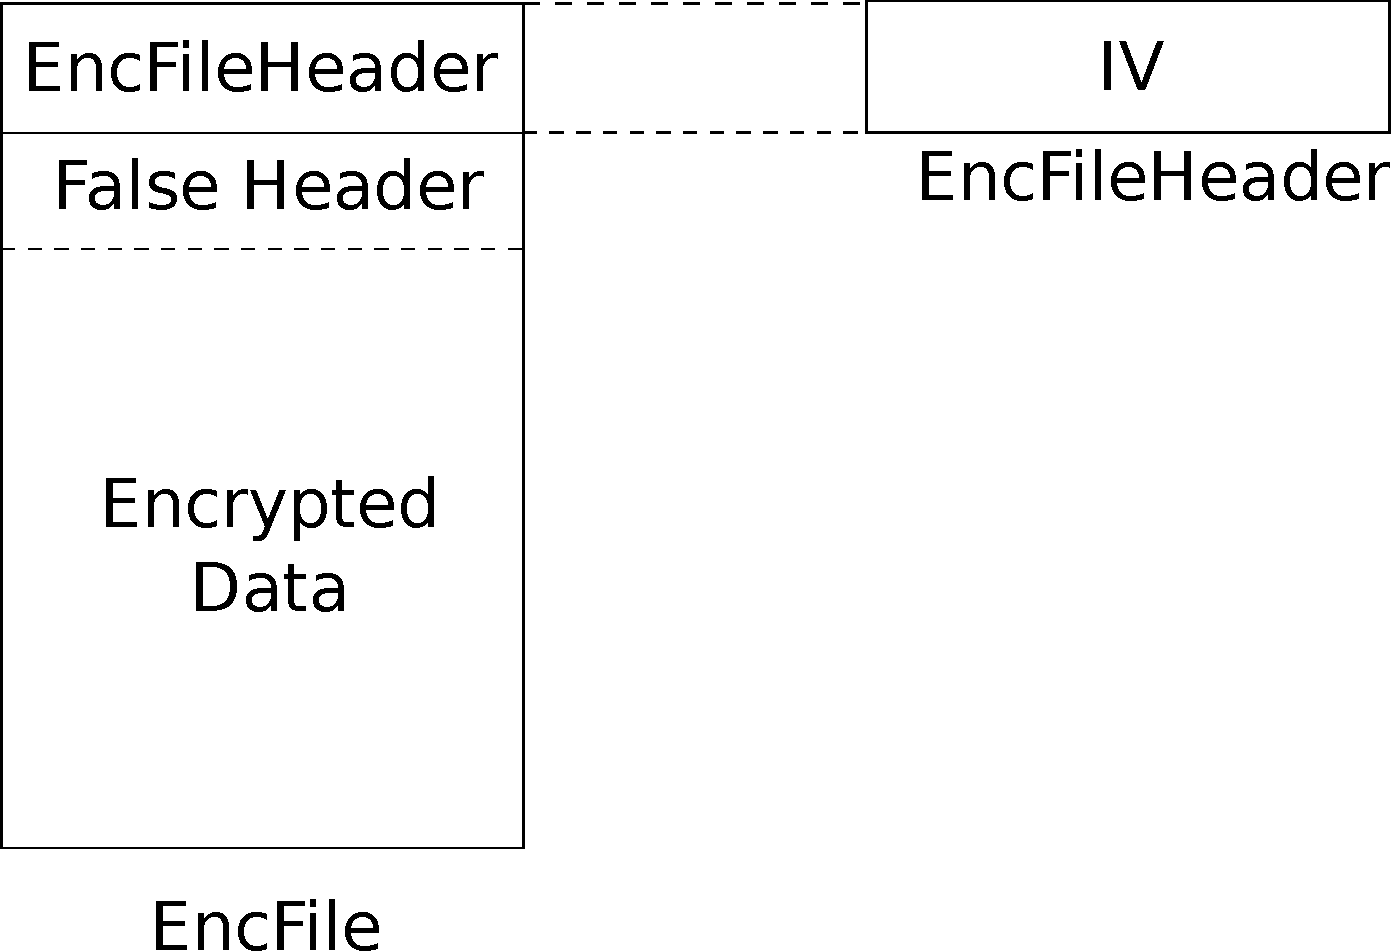
\includegraphics[scale=0.4]{Figures/EncFile_Header_1}
  \decoRule
  \caption[\code{EncFile} - \code{EncFileHeader} (Versión 1)]{Esquema general de las clases \code{EncFile} y \code{EncFileHeader} (Versión 1)}
  \label{fig:EncFile_Header_1}
\end{figure}

\begin{itemize}
  \item \keyword{\code{EncFile}} -- Viene a ser un objeto de clase \code{Slice} cifrado. A parte de los datos encriptados del \code{Slice}, también incluye una cabecera (\code{EncFileHeader}) con algunos datos importantes y una pseudocabecera (\code{FalseHeader}) con datos menores. (Figura~\ref{fig:EncFile_Header_1})

  \item \keyword{\code{EncFileHeader}} -- Esta cabecera se usa para almacenar algunos metadatos importantes como, en este caso, el vector de inicialización (IV) que se ha usado en el cifrado del objeto \code{Slice}. (Figura~\ref{fig:EncFile_Header_1})

  \item \keyword{\code{KeyFile}} -- Esta clase se utiliza para almacenar la clave simétrica que se ha utilizado para crear los objetos de clase \code{EncFile}.
\end{itemize}

Además de estas clases, se han creado otras clases que aportan los métodos necesarios para cifrar los fragmentos:

\begin{figure}[!htb]
  \centering
  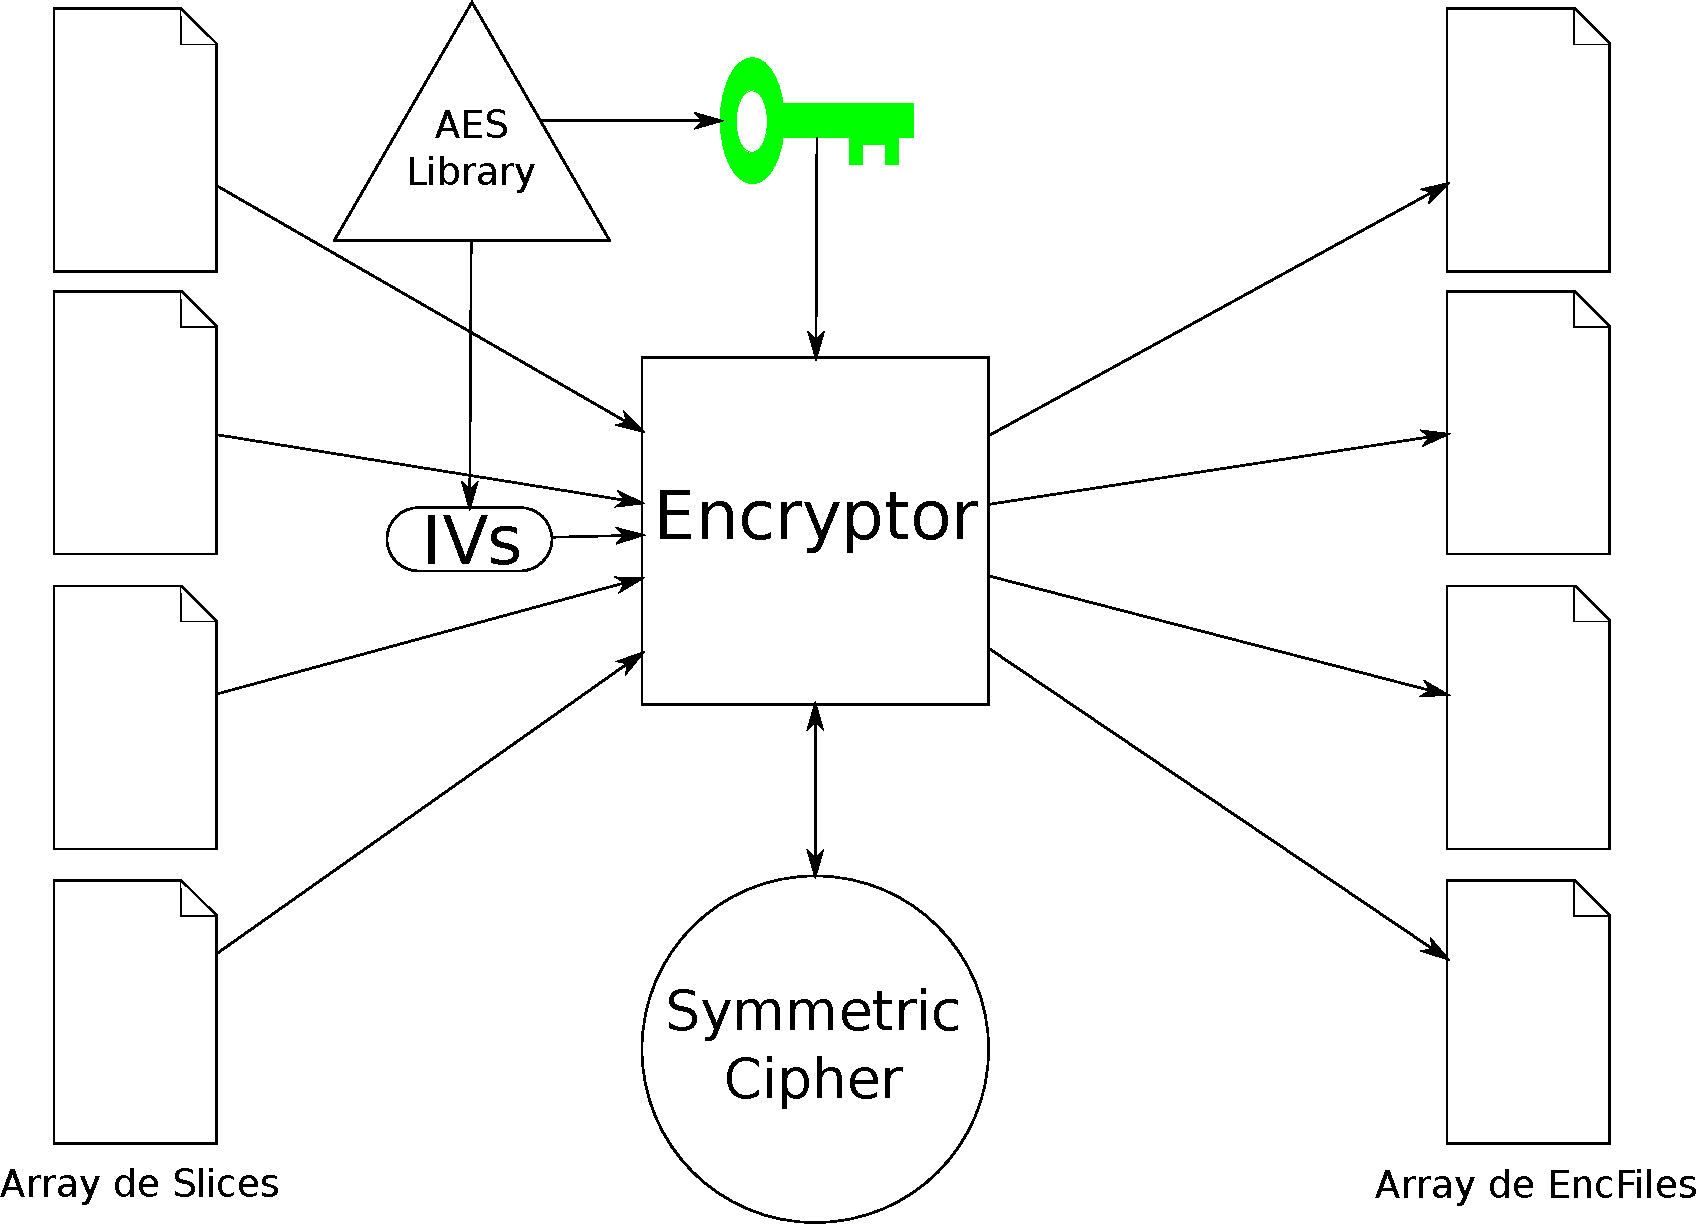
\includegraphics[scale=0.5]{Figures/Encryptor}
  \decoRule
  \caption[\code{Encryptor}]{Esquema general del funcionamiento de la clase \code{Encryptor}}
  \label{fig:Encryptor}
\end{figure}

\begin{figure}[!htb]
  \centering
  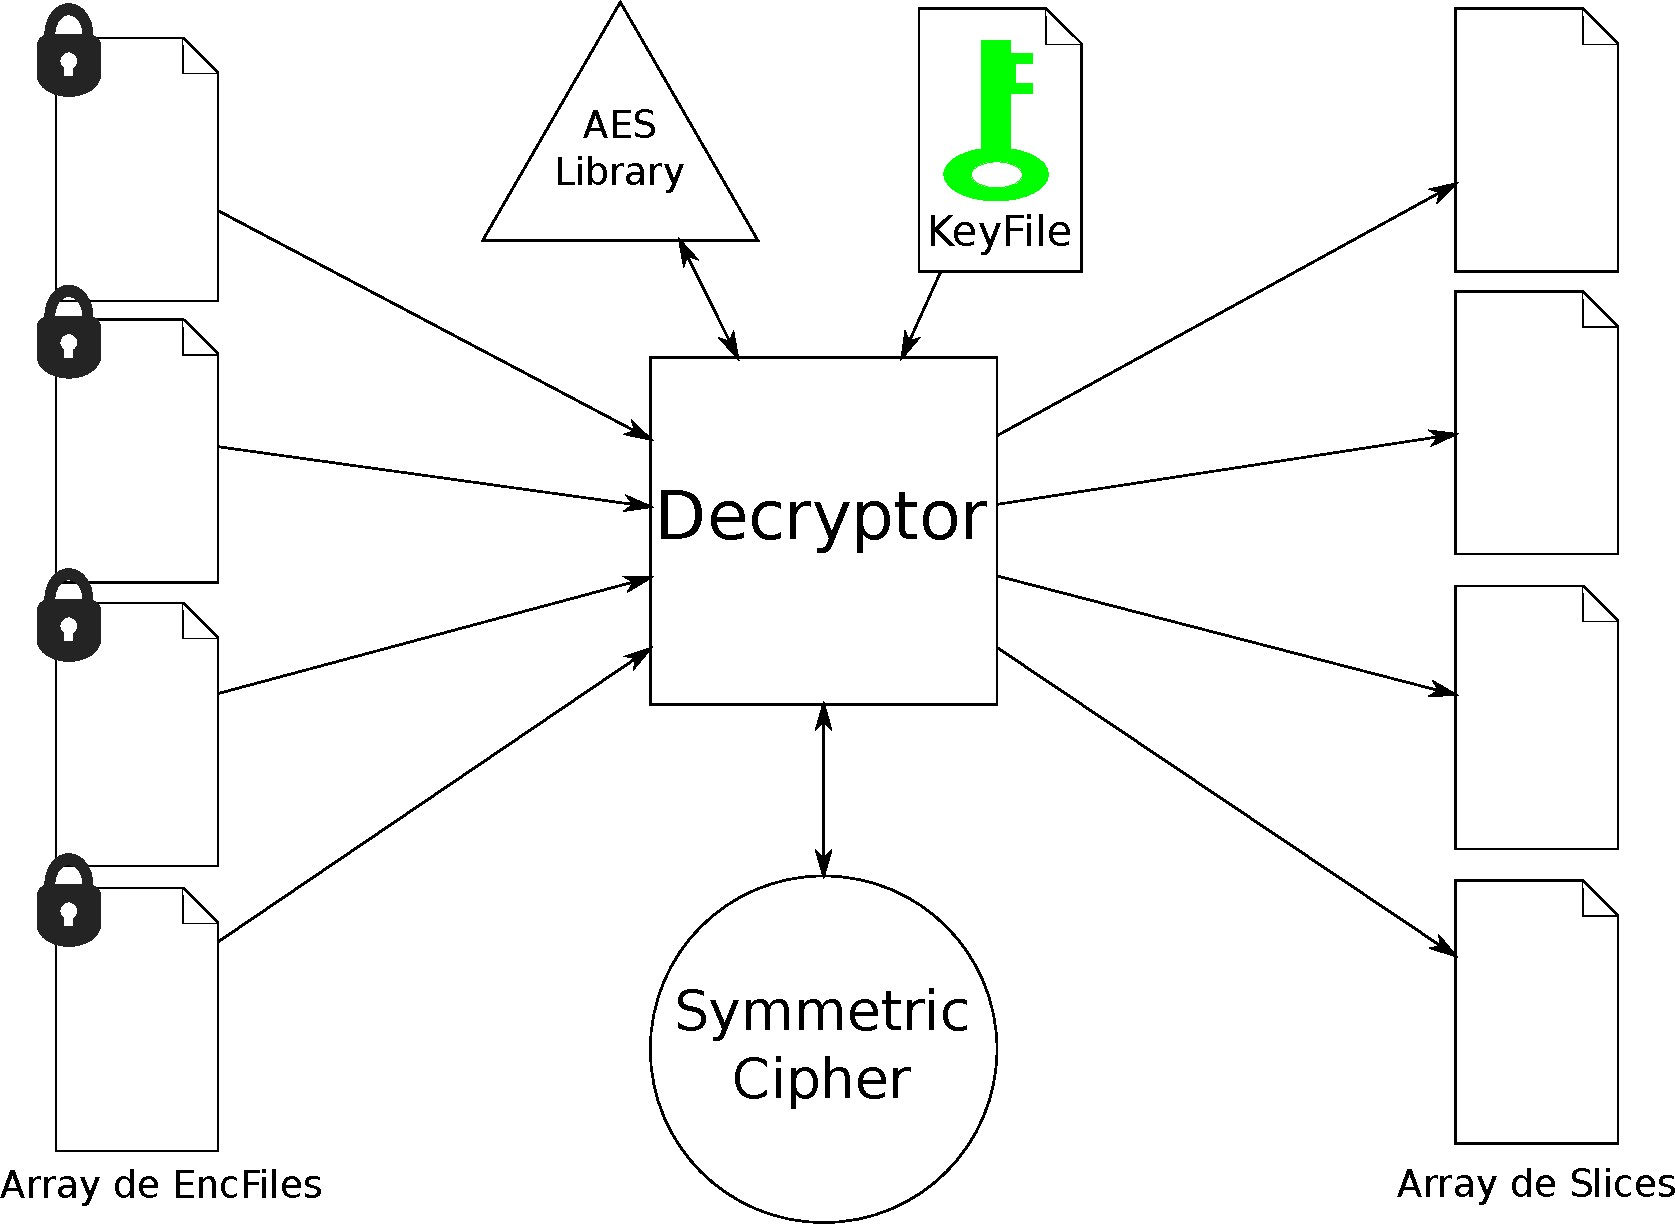
\includegraphics[scale=0.5]{Figures/Decryptor}
  \decoRule
  \caption[\code{Decryptor}]{Esquema general del funcionamiento de la clase \code{Decryptor}}
  \label{fig:Decryptor}
\end{figure}

\begin{itemize}
  \item \keyword{\code{AESLibrary}} -- Básicamente, una clase que se encarga de generar de manera aleatoria y segura claves simétricas y vectores de inicialización.

  \item \keyword{\code{SymmetricCipher}} -- Esta es la clase que se encarga de hacer la parte más importante en cuanto a la confidencialidad. Una vez que ha sido inicializada con una clave simétrica, genera textos cifrados a partir de texto plano y un IV. Igualmente, puede llevar a cabo el proceso inverso.

  \item \keyword{\code{Encryptor}} -- Esta clase, en conjunto con las dos anteriores, es la encargada de generar los objetos de clase \code{EncFile}. Genera de manera aleatoria y segura una clave simétrica para un algoritmo establecido y, con ella, inicializa una instancia de la clase \code{SymmetricCipher}. A continuación se le pasa un array de objetos de clase \code{Slice} del cual genera un array de objetos de clase \code{EncFile}, que es el que devuelve a través de un método. (Figura~\ref{fig:Encryptor})

  \item \keyword{\code{Decryptor}} -- La contraparte de la clase \code{Encryptor}. Realiza el proceso inverso y devuelve un array de objetos de clase \code{Slice} a partir de uno de objetos de clase \code{EncFile}. (Figura~\ref{fig:Decryptor})
\end{itemize}

\subsection{Shatter III}

El objetivo en esta tercera iteración es el de proporcionar integridad y autenticación a las clases ya implementadas, al igual que confidencialidad a la clave simétrica que se utiliza para generarlas. Para lograrlo, se han implementado algunas clases nuevas:

\begin{itemize}
  \item \keyword{\code{EncKeyFile}} -- Esta clase almacena la clave simétrica protegida mediante cifrado asimétrico usando la clave pública del destinatario del mensaje, con lo que se logra la confidencialidad de la clave entre los usuarios. Tiene una cabecera (\code{EncKeyFileHeader}) en la que se guardan algunos datos importantes.

  \item \keyword{\code{EncKeyFileHeader}} -- La cabecera de un objeto de clase \code{EncKeyFile}. En ella se almacena una HMAC cifrada de la clave simétrica.

  \item \keyword{\code{Signature}} -- Básicamente una clase para contener una HMAC.

  \item \keyword{\code{SecureSignature}} -- Contiene la HMAC comentada antes pero cifrada usando una clave asimétrica. De esta forma también le damos confidencialidad a la firma.
\end{itemize}

Para poder llevar a cabo el cifrado asimétrico se han desarrollado otras clases:

\begin{figure}[!htb]
  \centering
  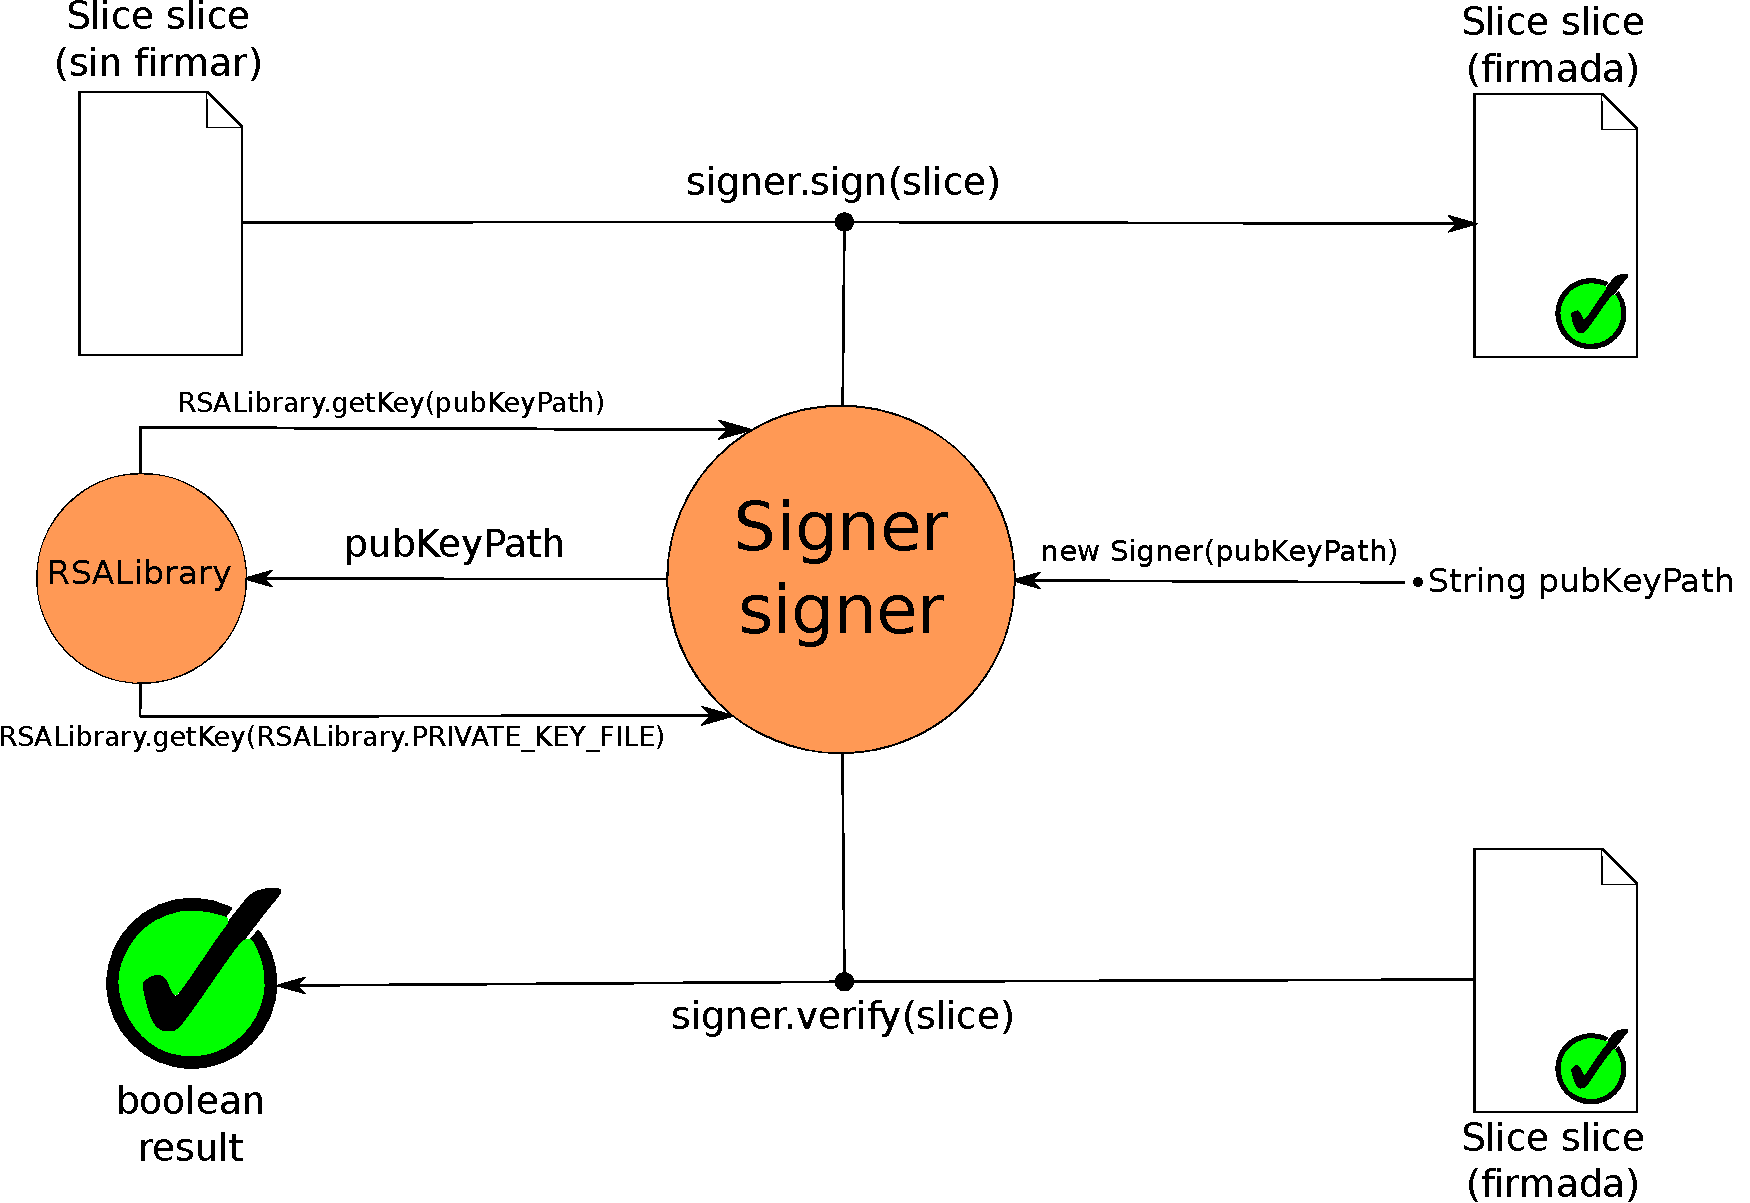
\includegraphics[scale=0.5]{Figures/Signer_1}
  \decoRule
  \caption[\code{Signer} (Versión 1)]{Esquema general del funcionamiento de la clase \code{Signer} (Versión 1)}
  \label{fig:Signer_1}
\end{figure}

\begin{itemize}
  \item \keyword{\code{RSALibrary}} -- Esta clase es la encargada de generar un par de claves asimétricas, de escribirlas y leerlas de un fichero, de cifrar un texto plano y de descifrar uno cifrado.

  \item \keyword{\code{Signer}} -- La clase que se encarga de recibir objetos de clase \code{Slice}, \code{EncFile}, \code{KeyFile} y demás y devolverlos firmados. Asimismo, se encarga de comprobar las firmas de todas estas clases para preservar la autenticidad de la información que portan. (Figura~\ref{fig:Signer_1})

  \item \keyword{\code{RSAPSS}} -- Esta clase incorpora todos los métodos necesarios para generar, a partir de un texto plano, un texto codificado y firmado usando el algoritmo RSASSA-PSS. También realiza el proceso inverso y puede verificar las firmas.
\end{itemize}

En este prototipo se ha añadido una firma a varias de las clases que ya estaban implementadas:

\begin{figure}[!htb]
  \centering
  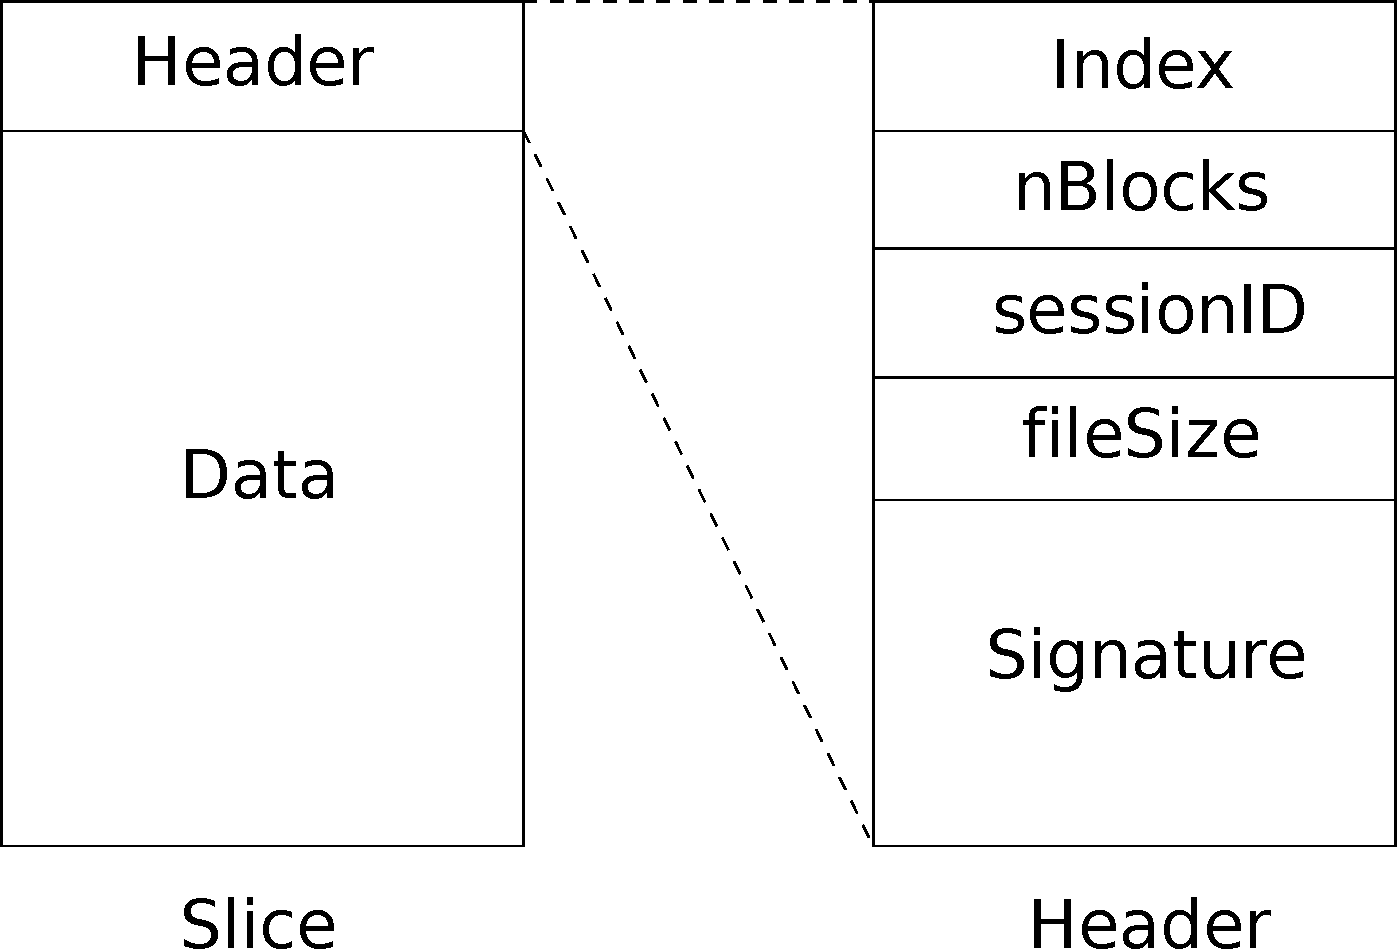
\includegraphics[scale=0.4]{Figures/Slice_Header_2}
  \decoRule
  \caption[\code{Slice} - \code{Header} (Versión final)]{Esquema general de las clases \code{Slice} y \code{Header} (Versión final)}
  \label{fig:Slice_Header_2}
\end{figure}

\begin{figure}[!htb]
  \centering
  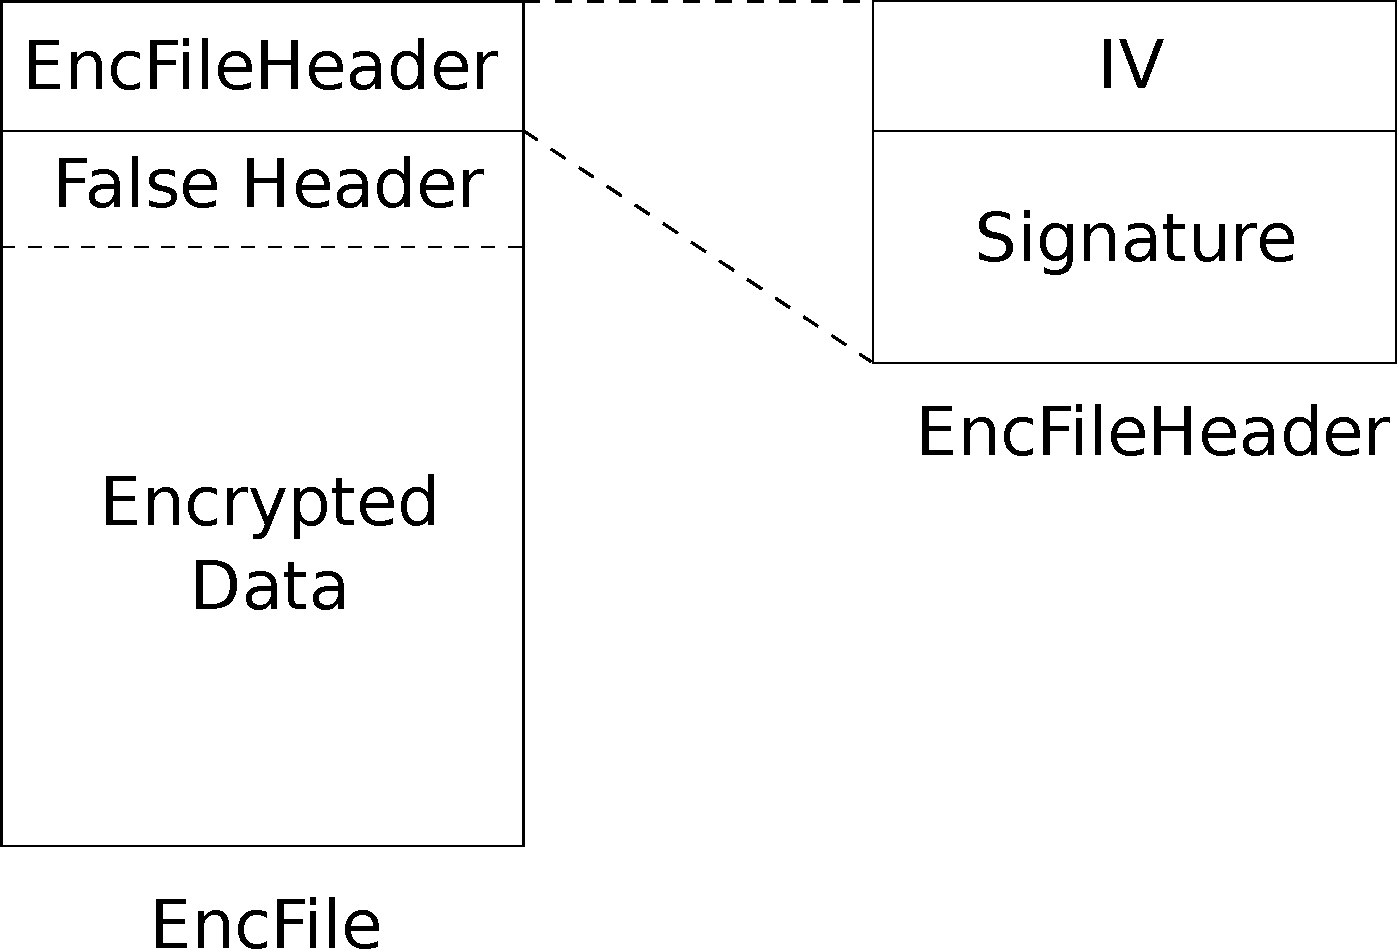
\includegraphics[scale=0.4]{Figures/EncFile_Header_2}
  \decoRule
  \caption[\code{EncFile} - \code{EncFileHeader} (Versión final)]{Esquema general de las clases \code{EncFile} y \code{EncFileHeader} (Versión final)}
  \label{fig:EncFile_Header_2}
\end{figure}

\begin{itemize}
  \item A la clase \code{Slice} se le ha añadido en la cabecera una firma, que otorga integridad y autenticación a los datos que lleva. (Figura~\ref{fig:Slice_Header_2})

  \item A la clase \code{EncFile} se le ha añadido también una firma, esta vez para darle la integridad y la autenticación al IV que se encuentra en su cabecera. (Figura~\ref{fig:EncFile_Header_2})

  \item La clase \code{KeyFile} tiene una firma de la clave simétrica.
\end{itemize}

Además de las clases mencionadas anteriormente, también se han desarrollado otras clases funcionales:

\begin{itemize}
  \item \keyword{\code{RandomString}} -- Esta clase posee un método que devuelve un \code{String} aleatorio de 8 caracteres.

  \item \keyword{\code{FileIO}} -- Esta clase tiene métodos para escribir y leer los distintos ficheros que intervienen en la aplicación.

  \item \keyword{\code{Bytes}} -- Tiene implementados varios métodos para hacer operaciones con arrays de \emph{bytes}.
\end{itemize}

\subsection{Shatter IV}

Este último prototipo está desarrollado como una aplicación en Android. El objetivo de este prototipo es hacer uso de varias herramientas que posee Android para que la aplicación funcione correctamente. Para ello se han creado nuevas clases:

\begin{itemize}
  \item \keyword{\code{KeyStoreHandler}} -- Esta clase se usa para realizar todas las operaciones necesarias con el \emph{Keystore} de Android (Véase~\ref{Keystore}). Se encarga de almacenar las claves, recuperarlas, usarlas para encriptar, firmar, etc.

  \item \keyword{\code{HTTPClient}} -- Un cliente HTTP muy sencillo que únicamente realiza peticiones GET.

  \item \keyword{\code{ExternalStorage}} -- Esta clase se encarga de interactuar con el \emph{External Storage} de Android. Incorpora algunos métodos para conseguir \emph{paths}, descriptores de fichero o crear directorios.
\end{itemize}

Para que los usuarios puedan enviar sus mensajes, se ha dispuesto un servidor HTTP bastante sencillo al que los usuarios pueden subir sus mensajes. Gracias a la clase \code{HTTPClient}, el destinatario puede bajarse los fragmentos de un mensaje.

\begin{figure}[!htb]
  \centering
  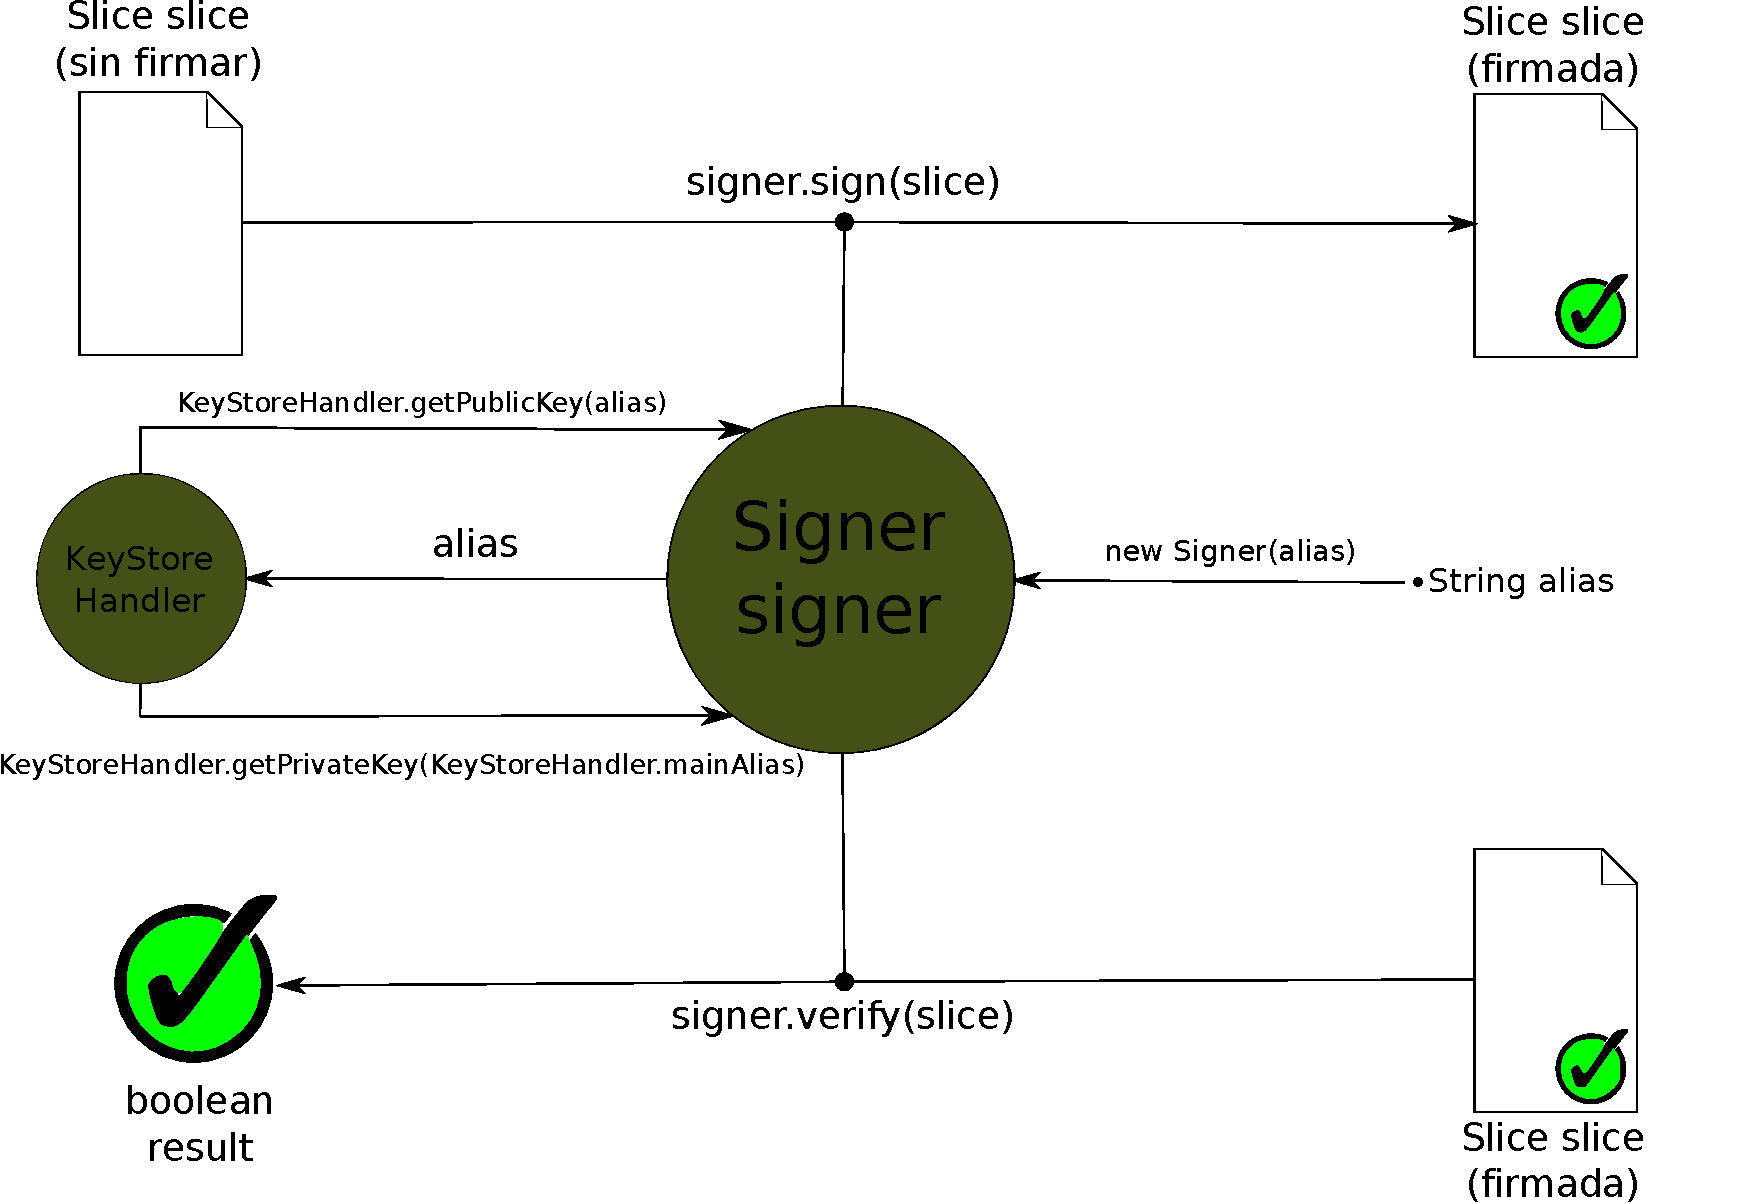
\includegraphics[scale=0.5]{Figures/Signer_2}
  \decoRule
  \caption[\code{Signer} (Versión final)]{Esquema general del funcionamiento de la clase \code{Signer} (Versión final)}
  \label{fig:Signer_2}
\end{figure}

El uso del \emph{Keystore} de Android obliga a utilizar las claves que se almacenan en él usando unos métodos específicos. Debido a ello, algunas clases ya creadas (Como \code{RSALibrary} o \code{RSAPSS}) se sustituyen por métodos específicos que se implementan en la clase \code{KeyStoreHandler}. (Figura~\ref{fig:Signer_2})

El ID que aparece en las cabeceras de la clase \code{Slice} se sustituye por un \code{String} aleatorio que genera la clase \code{RandomString}. Este cambio se debe a que el resumen \emph{hash} que se usaba anteriormente queda en desuso al añadir la firma a estas clases. Además, este ID aleatorio identifica a todos los objetos de clase \code{Slice} que pertenecen a un mismo mensaje.

El esquema general de la aplicación se puede dividir en dos: Una primera parte se encarga de la división y cifrado del fichero (Figura~\ref{fig:abstractA}). La otra se encarga de descargar del servidor los fragmentos cifrados y recomponer el fichero original (Figura~\ref{fig:abstractB}).

\begin{figure}[!htb]
  \centering
  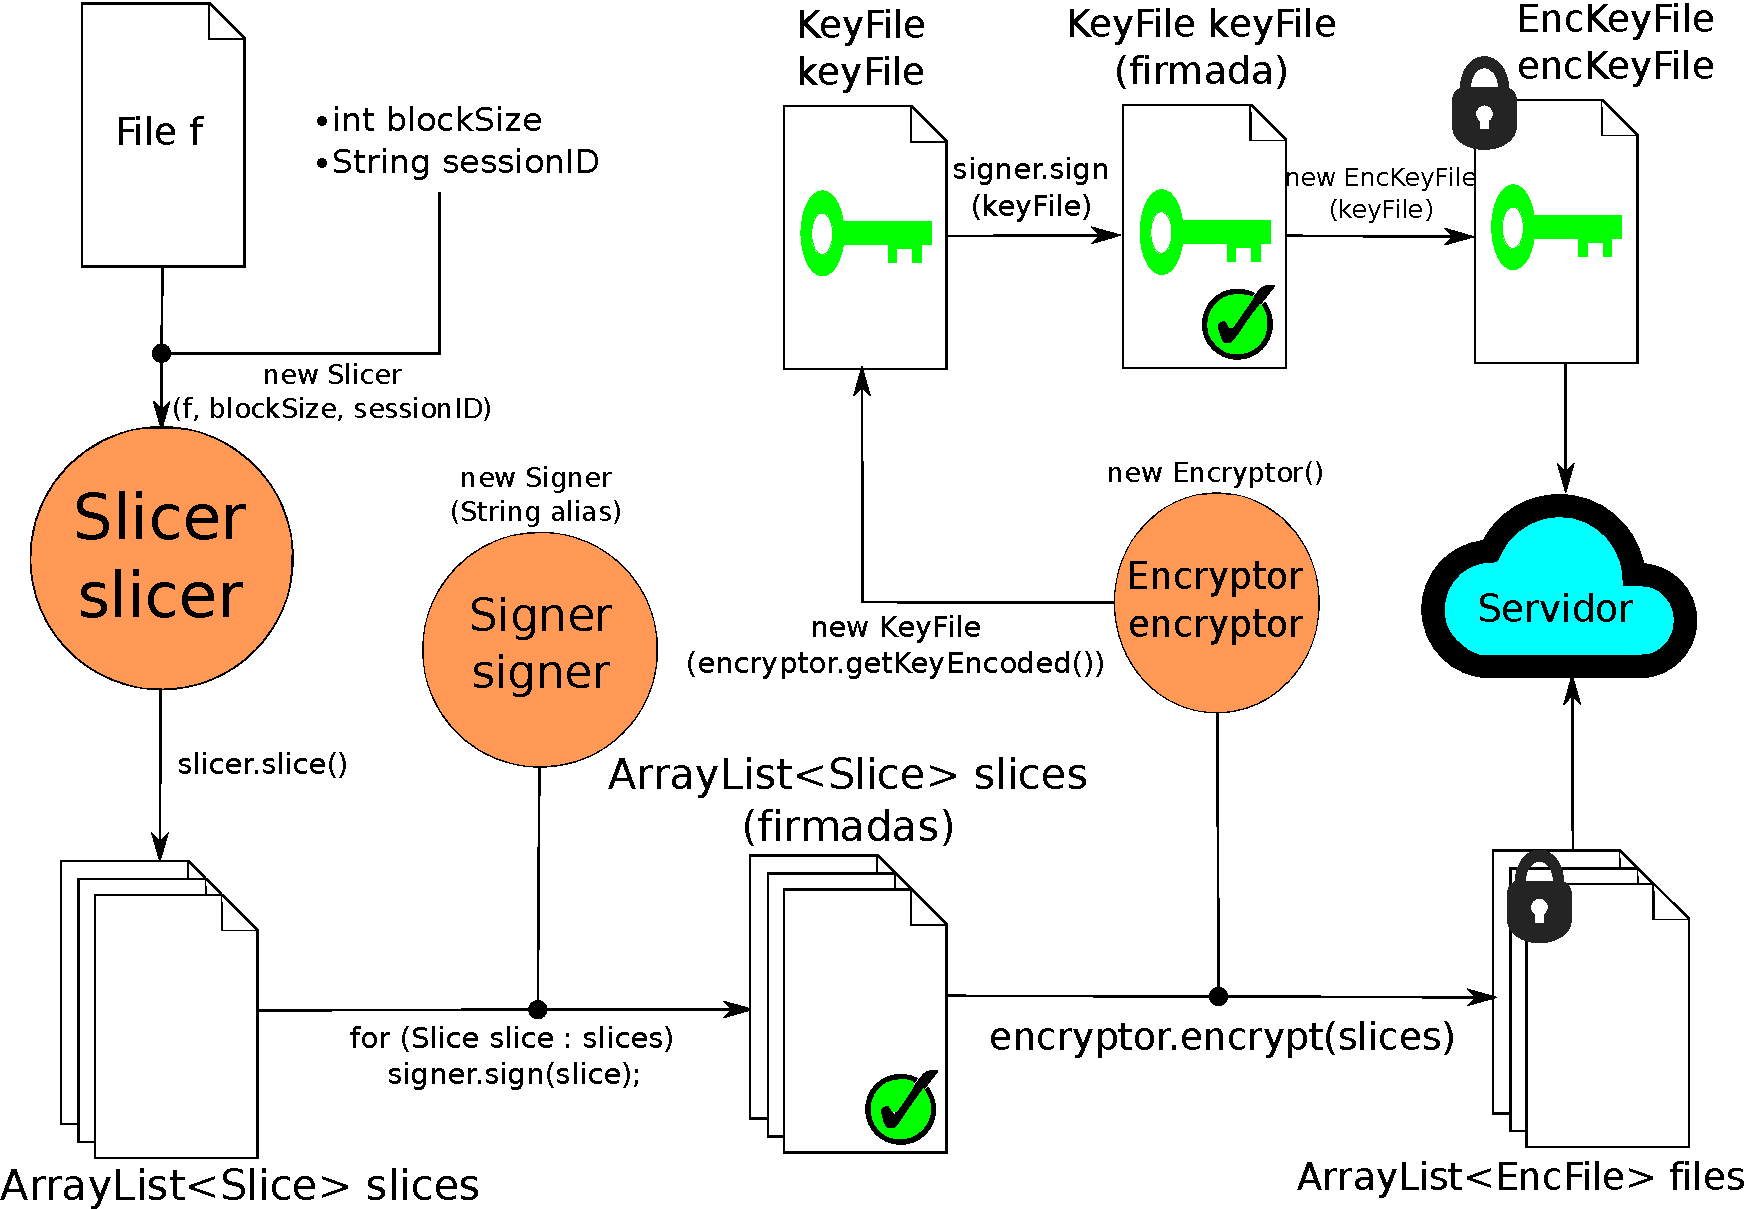
\includegraphics[scale=0.44]{Figures/abstractA}
  \decoRule
  \caption[\code{SliceEncrypt}]{Esquema general de la clase \code{SliceEncrypt}, la primera parte en el proceso de comunicación de la aplicación}
  \label{fig:abstractA}
\end{figure}

\begin{figure}[!htb]
  \centering
  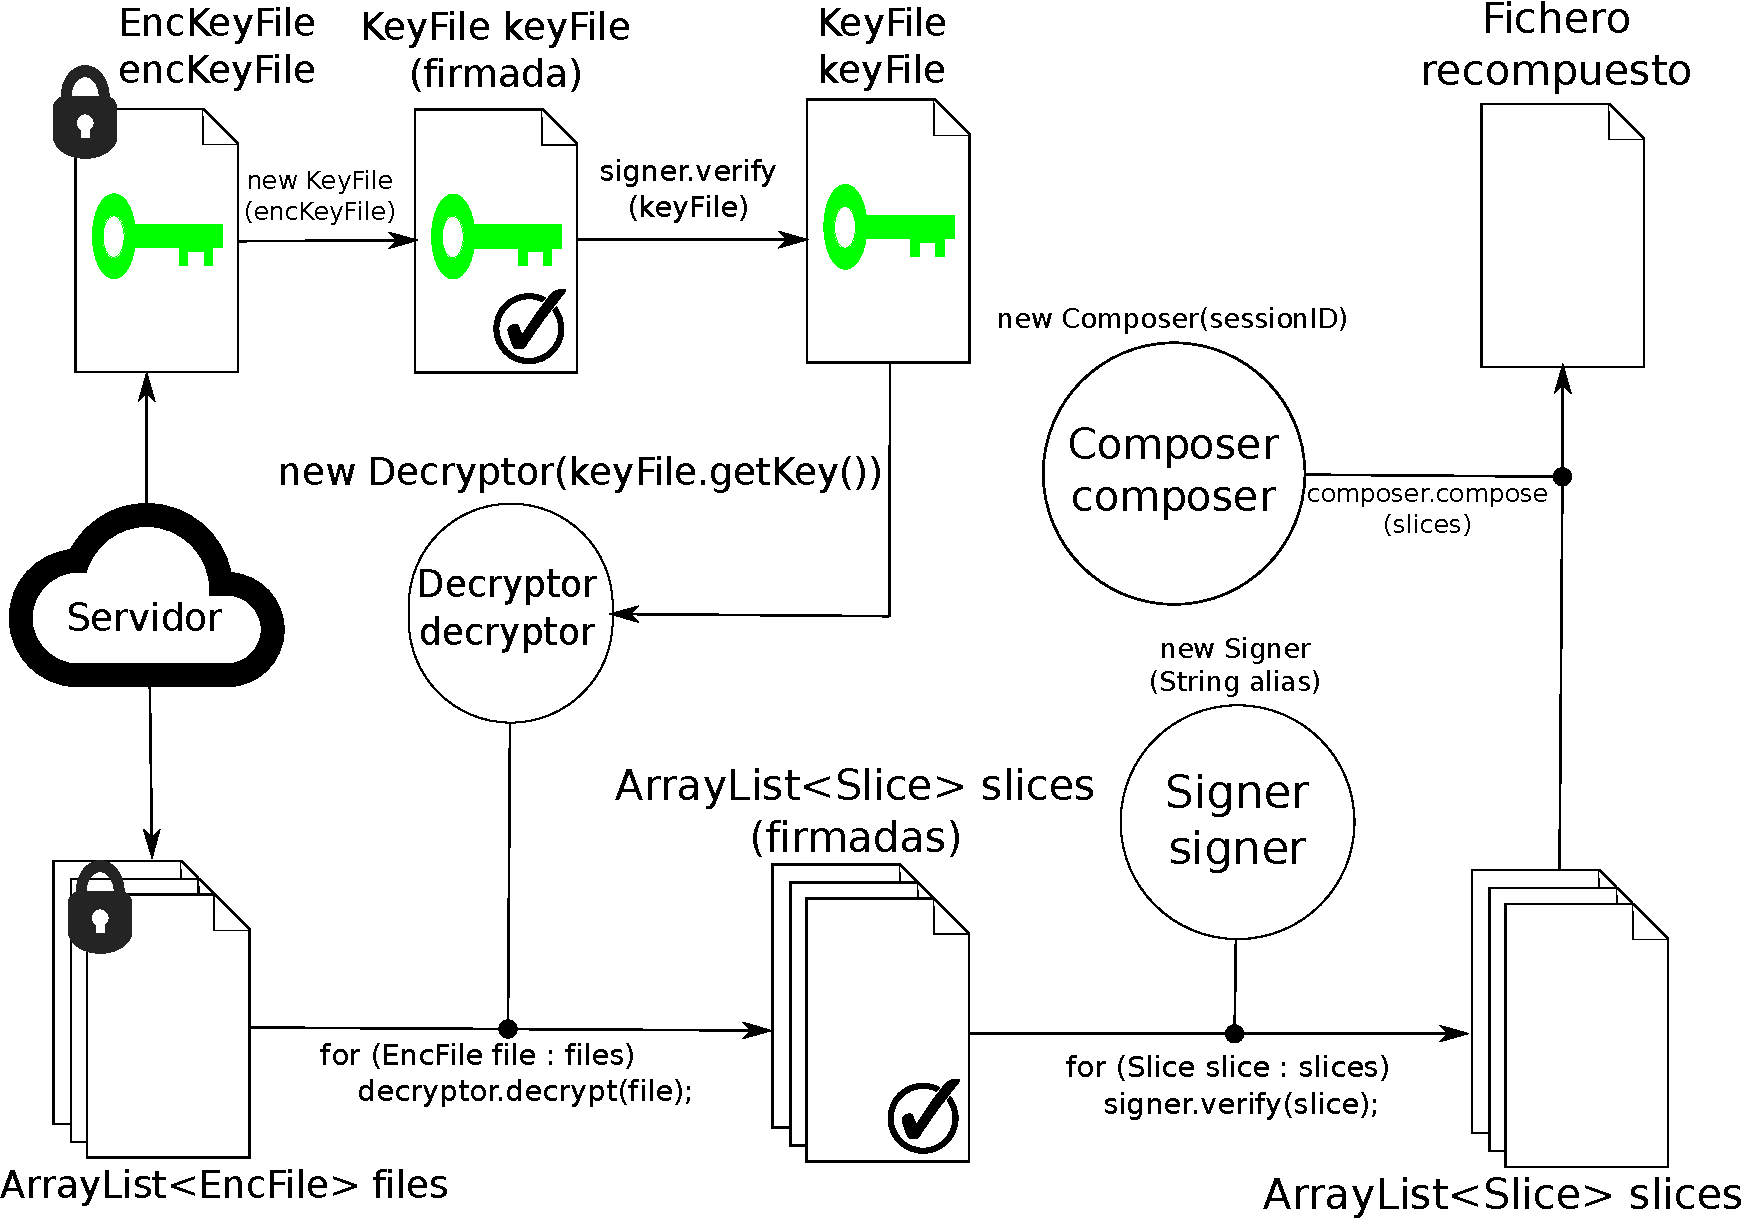
\includegraphics[scale=0.44]{Figures/abstractB}
  \decoRule
  \caption[\code{DecryptCompose}]{Esquema general de \code{DecryptCompose}, la parte final en el proceso de comunicación de la aplicación}
  \label{fig:abstractB}
\end{figure}

%-------------------------------------------------------------------------------

\section{Tiempo dedicado}

El desarrollo de cada prototipo ha necesitado un tiempo de trabajo distinto. En esta sección se detalla el número de horas dedicado a cada uno de ellos:

\begin{itemize}
  \item El primer prototipo, al tratarse de un esquema bastante sencillo, no ha supuesto un número de horas excesivo. El desarrollo de este prototipo se finalizó a las dos semanas de iniciar el proyecto, habiendo dedicado una media de dos horas diarias (28 horas).

  \item El segundo prototipo ha supuesto no solo tiempo de desarrollo, también ha necesitado tiempo de investigación para elegir el algoritmo más adecuado para el proyecto. Para este prototipo se dedicó, a partir de la finalización del prototipo anterior, dos semanas de desarrollo y una de investigación, dedicando una media de dos horas diarias (42 horas).

  \item El tercer prototipo ha necesitado una primera parte de investigación para elegir el algoritmo de cifrado asimétrico y firma adecuados y luego una parte de desarrollo. El desarrollo de este prototipo ha requerido, a partir de la finalización del prototipo anterior, dos semanas de investigación y cuatro de desarrollo, dedicando una media de dos horas diarias (84 horas).

  \item El cuarto prototipo, al tratarse de una migración a otra plataforma, no debería haber supuesto mucho tiempo de trabajo. Sin embargo se ha dedicado más tiempo debido a los problemas que se detallan en la Sección~\ref{Problemas encontrados}. Esta fase ha requerido una primera semana de investigación para encontrar la mejor forma de realizar la migración, y cinco semanas de desarrollo para llevarlo a cabo, dedicando una media de dos horas diarias (84 horas).
\end{itemize}

En total, el desarrollo del proyecto ha conllevado aproximadamente 238 horas de trabajo, habiendo invertido más tiempo en el desarrollo que en la investigación.
